% Armónicos esféricos Y_l^m en la esfera S^2
% Compilar con: pdflatex spherical_harmonics.tex
\documentclass[tikz,border=10pt]{standalone}
\usepackage{tikz}
\usepackage{amsmath,amssymb}
\usetikzlibrary{calc}

\definecolor{gdlblue}{RGB}{41, 98, 168}
\definecolor{gdlred}{RGB}{191, 49, 49}
\definecolor{gdlgreen}{RGB}{30, 130, 76}
\definecolor{gdlorange}{RGB}{217, 130, 30}
\definecolor{gdlpurple}{RGB}{118, 56, 138}
\definecolor{gdlgray}{RGB}{140, 140, 140}
\definecolor{gdlyellow}{RGB}{190, 140, 10}

\begin{document}
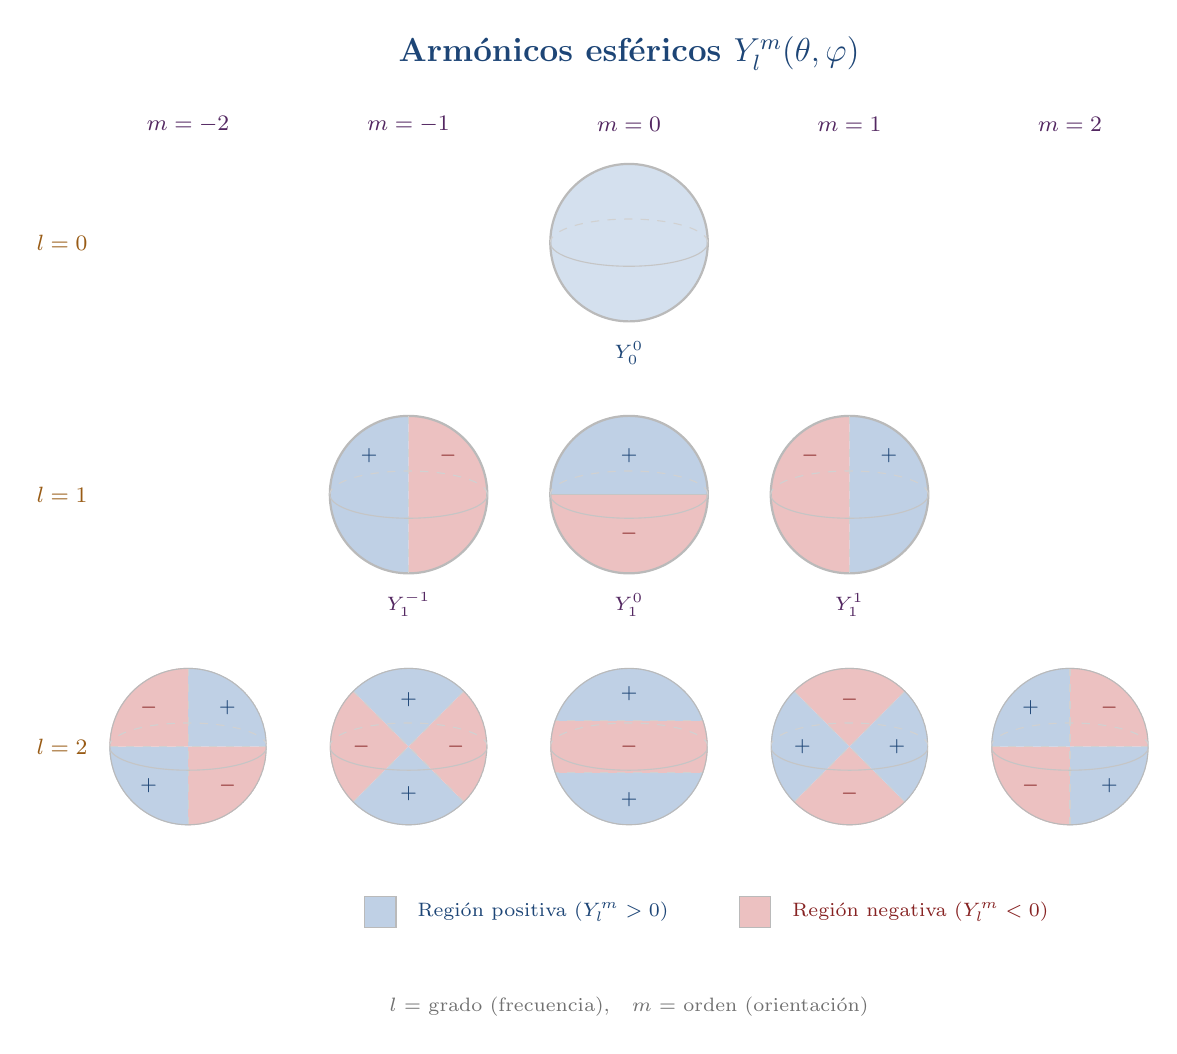
\begin{tikzpicture}[
    every node/.style={font=\small}
  ]

  \def\sphR{1}       % sphere radius
  \def\colsep{2.8}   % horizontal spacing between columns
  \def\rowsep{3.2}   % vertical spacing between rows

  % Coordinate origin: column m=0 is at x = 2*\colsep, row l=0 at y = 0

  % ============================================================
  % Title
  % ============================================================
  \node[font=\large\bfseries, text=gdlblue!70!black]
    at ({2*\colsep}, 2.4) {Arm\'onicos esf\'ericos $Y_l^m(\theta,\varphi)$};

  % ============================================================
  % Column headers (m values) — placed well above the l=0 sphere
  % ============================================================
  \foreach \m/\col in {-2/0, -1/1, 0/2, 1/3, 2/4} {
    \node[font=\footnotesize, text=gdlpurple!70!black] at ({\col*\colsep}, 1.5)
      {$m = \m$};
  }

  % ============================================================
  % Row labels (l values) — centered vertically with each row
  % ============================================================
  \node[font=\footnotesize, text=gdlorange!70!black] at (-1.6, 0)         {$l = 0$};
  \node[font=\footnotesize, text=gdlorange!70!black] at (-1.6, -\rowsep)  {$l = 1$};
  \node[font=\footnotesize, text=gdlorange!70!black] at (-1.6, -2*\rowsep){$l = 2$};

  % ============================================================
  % Helper macro: draw equator ellipse on a sphere
  % ============================================================
  % (drawn after fills so it sits on top)

  % ============================================================
  % l = 0, m = 0 : Y_0^0 — constant function, uniform positive
  % ============================================================
  \begin{scope}[shift={(2*\colsep, 0)}]
    \fill[gdlblue!20] (0,0) circle (\sphR);
    \draw[gdlgray!60, thick] (0,0) circle (\sphR);
    % equator ellipse
    \draw[gdlgray!40, dashed] ({\sphR},0)
      arc[start angle=0, end angle=180, x radius=\sphR, y radius=0.3*\sphR];
    \draw[gdlgray!50] ({-\sphR},0)
      arc[start angle=180, end angle=360, x radius=\sphR, y radius=0.3*\sphR];
    \node[font=\scriptsize, text=gdlblue!70!black] at (0, -\sphR - 0.4) {$Y_0^0$};
  \end{scope}

  % ============================================================
  % l = 1, m = -1 : Y_1^{-1} — left/right split
  % ============================================================
  \begin{scope}[shift={(1*\colsep, -\rowsep)}]
    \fill[gdlblue!30] (90:\sphR) arc (90:270:\sphR) -- cycle;
    \fill[gdlred!30]  (90:\sphR) arc (90:-90:\sphR) -- cycle;
    \draw[gdlgray!60, thick] (0,0) circle (\sphR);
    \draw[gdlgray!40, dashed] (0,\sphR) -- (0,-\sphR);
    % equator
    \draw[gdlgray!40, dashed] ({\sphR},0)
      arc[start angle=0, end angle=180, x radius=\sphR, y radius=0.3*\sphR];
    \draw[gdlgray!50] ({-\sphR},0)
      arc[start angle=180, end angle=360, x radius=\sphR, y radius=0.3*\sphR];
    \node[font=\scriptsize, text=gdlblue!70!black] at (-0.5, 0.5) {$+$};
    \node[font=\scriptsize, text=gdlred!70!black]  at ( 0.5, 0.5) {$-$};
    \node[font=\scriptsize, text=gdlpurple!70!black] at (0, -\sphR - 0.4) {$Y_1^{-1}$};
  \end{scope}

  % ============================================================
  % l = 1, m = 0 : Y_1^0 — top/bottom split (zonal)
  % ============================================================
  \begin{scope}[shift={(2*\colsep, -\rowsep)}]
    \fill[gdlblue!30] (-\sphR,0) arc (180:0:\sphR) -- cycle;
    \fill[gdlred!30]  (-\sphR,0) arc (180:360:\sphR) -- cycle;
    \draw[gdlgray!60, thick] (0,0) circle (\sphR);
    \draw[gdlgray!50] (-\sphR,0) -- (\sphR,0);
    % equator
    \draw[gdlgray!40, dashed] ({\sphR},0)
      arc[start angle=0, end angle=180, x radius=\sphR, y radius=0.3*\sphR];
    \draw[gdlgray!50] ({-\sphR},0)
      arc[start angle=180, end angle=360, x radius=\sphR, y radius=0.3*\sphR];
    \node[font=\scriptsize, text=gdlblue!70!black] at (0,  0.5) {$+$};
    \node[font=\scriptsize, text=gdlred!70!black]  at (0, -0.5) {$-$};
    \node[font=\scriptsize, text=gdlpurple!70!black] at (0, -\sphR - 0.4) {$Y_1^{0}$};
  \end{scope}

  % ============================================================
  % l = 1, m = 1 : Y_1^1 — left/right split (opposite of Y_1^{-1})
  % ============================================================
  \begin{scope}[shift={(3*\colsep, -\rowsep)}]
    \fill[gdlred!30]  (90:\sphR) arc (90:270:\sphR) -- cycle;
    \fill[gdlblue!30] (90:\sphR) arc (90:-90:\sphR) -- cycle;
    \draw[gdlgray!60, thick] (0,0) circle (\sphR);
    \draw[gdlgray!40, dashed] (0,\sphR) -- (0,-\sphR);
    % equator
    \draw[gdlgray!40, dashed] ({\sphR},0)
      arc[start angle=0, end angle=180, x radius=\sphR, y radius=0.3*\sphR];
    \draw[gdlgray!50] ({-\sphR},0)
      arc[start angle=180, end angle=360, x radius=\sphR, y radius=0.3*\sphR];
    \node[font=\scriptsize, text=gdlred!70!black]  at (-0.5, 0.5) {$-$};
    \node[font=\scriptsize, text=gdlblue!70!black] at ( 0.5, 0.5) {$+$};
    \node[font=\scriptsize, text=gdlpurple!70!black] at (0, -\sphR - 0.4) {$Y_1^{1}$};
  \end{scope}

  % ============================================================
  % l = 2, m = -2 : Y_2^{-2} — axis-aligned quadrants
  % ============================================================
  \begin{scope}[shift={(0*\colsep, -2*\rowsep)}]
    \clip (0,0) circle (\sphR);
    \fill[gdlblue!30] (0,0) -- (90:\sphR)  arc (90:0:\sphR)    -- cycle;
    \fill[gdlred!30]  (0,0) -- (0:\sphR)   arc (0:-90:\sphR)   -- cycle;
    \fill[gdlblue!30] (0,0) -- (-90:\sphR) arc (-90:-180:\sphR) -- cycle;
    \fill[gdlred!30]  (0,0) -- (180:\sphR) arc (180:90:\sphR)  -- cycle;
    \draw[gdlgray!40, dashed] (-\sphR,0) -- (\sphR,0);
    \draw[gdlgray!40, dashed] (0,-\sphR) -- (0,\sphR);
    \draw[gdlgray!60, thick] (0,0) circle (\sphR);
    % equator
    \draw[gdlgray!40, dashed] ({\sphR},0)
      arc[start angle=0, end angle=180, x radius=\sphR, y radius=0.3*\sphR];
    \draw[gdlgray!50] ({-\sphR},0)
      arc[start angle=180, end angle=360, x radius=\sphR, y radius=0.3*\sphR];
    \node[font=\scriptsize, text=gdlblue!70!black] at ( 0.5,  0.5) {$+$};
    \node[font=\scriptsize, text=gdlred!70!black]  at ( 0.5, -0.5) {$-$};
    \node[font=\scriptsize, text=gdlblue!70!black] at (-0.5, -0.5) {$+$};
    \node[font=\scriptsize, text=gdlred!70!black]  at (-0.5,  0.5) {$-$};
    \node[font=\scriptsize, text=gdlpurple!70!black] at (0, -\sphR - 0.4) {$Y_2^{-2}$};
  \end{scope}

  % ============================================================
  % l = 2, m = -1 : Y_2^{-1} — diagonal quadrants
  % ============================================================
  \begin{scope}[shift={(1*\colsep, -2*\rowsep)}]
    \clip (0,0) circle (\sphR);
    \fill[gdlblue!30] (0,0) -- (45:\sphR)  arc (45:135:\sphR)  -- cycle;
    \fill[gdlred!30]  (0,0) -- (135:\sphR) arc (135:225:\sphR) -- cycle;
    \fill[gdlblue!30] (0,0) -- (225:\sphR) arc (225:315:\sphR) -- cycle;
    \fill[gdlred!30]  (0,0) -- (315:\sphR) arc (315:405:\sphR) -- cycle;
    \draw[gdlgray!40, dashed] ({-0.71*\sphR},{-0.71*\sphR}) -- ({0.71*\sphR},{0.71*\sphR});
    \draw[gdlgray!40, dashed] ({-0.71*\sphR},{0.71*\sphR})  -- ({0.71*\sphR},{-0.71*\sphR});
    \draw[gdlgray!60, thick] (0,0) circle (\sphR);
    % equator
    \draw[gdlgray!40, dashed] ({\sphR},0)
      arc[start angle=0, end angle=180, x radius=\sphR, y radius=0.3*\sphR];
    \draw[gdlgray!50] ({-\sphR},0)
      arc[start angle=180, end angle=360, x radius=\sphR, y radius=0.3*\sphR];
    \node[font=\scriptsize, text=gdlblue!70!black] at (0,  0.6) {$+$};
    \node[font=\scriptsize, text=gdlred!70!black]  at (-0.6, 0) {$-$};
    \node[font=\scriptsize, text=gdlblue!70!black] at (0, -0.6) {$+$};
    \node[font=\scriptsize, text=gdlred!70!black]  at ( 0.6, 0) {$-$};
    \node[font=\scriptsize, text=gdlpurple!70!black] at (0, -\sphR - 0.4) {$Y_2^{-1}$};
  \end{scope}

  % ============================================================
  % l = 2, m = 0 : Y_2^0 — three horizontal bands (zonal)
  % ============================================================
  \begin{scope}[shift={(2*\colsep, -2*\rowsep)}]
    \clip (0,0) circle (\sphR);
    \fill[gdlblue!30] (-\sphR, {0.33*\sphR}) rectangle (\sphR, \sphR);
    \fill[gdlred!30]  (-\sphR, {-0.33*\sphR}) rectangle (\sphR, {0.33*\sphR});
    \fill[gdlblue!30] (-\sphR, -\sphR) rectangle (\sphR, {-0.33*\sphR});
    \draw[gdlgray!40, dashed] (-\sphR, {0.33*\sphR})  -- (\sphR, {0.33*\sphR});
    \draw[gdlgray!40, dashed] (-\sphR, {-0.33*\sphR}) -- (\sphR, {-0.33*\sphR});
    \draw[gdlgray!60, thick] (0,0) circle (\sphR);
    % equator
    \draw[gdlgray!40, dashed] ({\sphR},0)
      arc[start angle=0, end angle=180, x radius=\sphR, y radius=0.3*\sphR];
    \draw[gdlgray!50] ({-\sphR},0)
      arc[start angle=180, end angle=360, x radius=\sphR, y radius=0.3*\sphR];
    \node[font=\scriptsize, text=gdlblue!70!black] at (0,  0.67) {$+$};
    \node[font=\scriptsize, text=gdlred!70!black]  at (0,  0)    {$-$};
    \node[font=\scriptsize, text=gdlblue!70!black] at (0, -0.67) {$+$};
    \node[font=\scriptsize, text=gdlpurple!70!black] at (0, -\sphR - 0.4) {$Y_2^{0}$};
  \end{scope}

  % ============================================================
  % l = 2, m = 1 : Y_2^1 — diagonal quadrants (opposite of Y_2^{-1})
  % ============================================================
  \begin{scope}[shift={(3*\colsep, -2*\rowsep)}]
    \clip (0,0) circle (\sphR);
    \fill[gdlred!30]  (0,0) -- (45:\sphR)  arc (45:135:\sphR)  -- cycle;
    \fill[gdlblue!30] (0,0) -- (135:\sphR) arc (135:225:\sphR) -- cycle;
    \fill[gdlred!30]  (0,0) -- (225:\sphR) arc (225:315:\sphR) -- cycle;
    \fill[gdlblue!30] (0,0) -- (315:\sphR) arc (315:405:\sphR) -- cycle;
    \draw[gdlgray!40, dashed] ({-0.71*\sphR},{-0.71*\sphR}) -- ({0.71*\sphR},{0.71*\sphR});
    \draw[gdlgray!40, dashed] ({-0.71*\sphR},{0.71*\sphR})  -- ({0.71*\sphR},{-0.71*\sphR});
    \draw[gdlgray!60, thick] (0,0) circle (\sphR);
    % equator
    \draw[gdlgray!40, dashed] ({\sphR},0)
      arc[start angle=0, end angle=180, x radius=\sphR, y radius=0.3*\sphR];
    \draw[gdlgray!50] ({-\sphR},0)
      arc[start angle=180, end angle=360, x radius=\sphR, y radius=0.3*\sphR];
    \node[font=\scriptsize, text=gdlred!70!black]  at (0,  0.6) {$-$};
    \node[font=\scriptsize, text=gdlblue!70!black] at (-0.6, 0) {$+$};
    \node[font=\scriptsize, text=gdlred!70!black]  at (0, -0.6) {$-$};
    \node[font=\scriptsize, text=gdlblue!70!black] at ( 0.6, 0) {$+$};
    \node[font=\scriptsize, text=gdlpurple!70!black] at (0, -\sphR - 0.4) {$Y_2^{1}$};
  \end{scope}

  % ============================================================
  % l = 2, m = 2 : Y_2^2 — axis-aligned quadrants (opposite of Y_2^{-2})
  % ============================================================
  \begin{scope}[shift={(4*\colsep, -2*\rowsep)}]
    \clip (0,0) circle (\sphR);
    \fill[gdlred!30]  (0,0) -- (90:\sphR)  arc (90:0:\sphR)    -- cycle;
    \fill[gdlblue!30] (0,0) -- (0:\sphR)   arc (0:-90:\sphR)   -- cycle;
    \fill[gdlred!30]  (0,0) -- (-90:\sphR) arc (-90:-180:\sphR) -- cycle;
    \fill[gdlblue!30] (0,0) -- (180:\sphR) arc (180:90:\sphR)  -- cycle;
    \draw[gdlgray!40, dashed] (-\sphR,0) -- (\sphR,0);
    \draw[gdlgray!40, dashed] (0,-\sphR) -- (0,\sphR);
    \draw[gdlgray!60, thick] (0,0) circle (\sphR);
    % equator
    \draw[gdlgray!40, dashed] ({\sphR},0)
      arc[start angle=0, end angle=180, x radius=\sphR, y radius=0.3*\sphR];
    \draw[gdlgray!50] ({-\sphR},0)
      arc[start angle=180, end angle=360, x radius=\sphR, y radius=0.3*\sphR];
    \node[font=\scriptsize, text=gdlred!70!black]  at ( 0.5,  0.5) {$-$};
    \node[font=\scriptsize, text=gdlblue!70!black] at ( 0.5, -0.5) {$+$};
    \node[font=\scriptsize, text=gdlred!70!black]  at (-0.5, -0.5) {$-$};
    \node[font=\scriptsize, text=gdlblue!70!black] at (-0.5,  0.5) {$+$};
    \node[font=\scriptsize, text=gdlpurple!70!black] at (0, -\sphR - 0.4) {$Y_2^{2}$};
  \end{scope}

  % ============================================================
  % Legend
  % ============================================================
  \begin{scope}[shift={(0, {-2*\rowsep - 2.3})}]
    \fill[gdlblue!30] ({0.8*\colsep}, 0) rectangle ++(0.4, 0.4);
    \draw[gdlgray!60] ({0.8*\colsep}, 0) rectangle ++(0.4, 0.4);
    \node[font=\scriptsize, anchor=west, text=gdlblue!70!black]
      at ({0.8*\colsep + 0.55}, 0.2) {Regi\'on positiva ($Y_l^m > 0$)};

    \fill[gdlred!30] ({2.5*\colsep}, 0) rectangle ++(0.4, 0.4);
    \draw[gdlgray!60] ({2.5*\colsep}, 0) rectangle ++(0.4, 0.4);
    \node[font=\scriptsize, anchor=west, text=gdlred!70!black]
      at ({2.5*\colsep + 0.55}, 0.2) {Regi\'on negativa ($Y_l^m < 0$)};
  \end{scope}

  % ============================================================
  % Explanatory note
  % ============================================================
  \node[font=\scriptsize, text=gdlgray!80!black, text width=9cm, align=center]
    at ({2*\colsep}, {-2*\rowsep - 3.3})
    {$l$ = grado (frecuencia),\quad $m$ = orden (orientaci\'on)};

\end{tikzpicture}
\end{document}
